\subsection{Kiểm chứng toàn vẹn dữ liệu — Cây Merkle}

\subsubsection{Cấu trúc cây Merkle cam kết}

Khi cuộc bầu cử kết thúc, toàn bộ tập hợp cam kết phiếu (\textit{blinded commitment}) được tổng hợp thành một cây Merkle có gốc duy nhất. Mỗi lá là giá trị băm SHA-256 của chuỗi hex commit; các nút trong được tính bằng cách băm cặp con đã được sắp xếp theo thứ tự byte; gốc cây sau cùng là một giá trị 32 byte tóm tắt toàn bộ phiếu bầu trong bầu cử. Cấu trúc tổng quát được minh họa trong Hình~\ref{fig:merkle-tree}.

\begin{figure}[H]
    \centering
    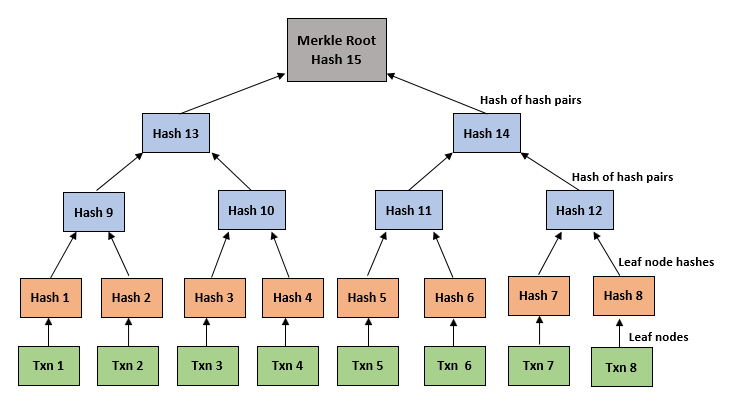
\includegraphics[width=0.6\textwidth, keepaspectratio]{Figures/Merkle-tree.png}
    \caption{Cây Merkle cam kết được sinh ra khi đóng bầu cử}
    \label{fig:merkle-tree}
\end{figure}

Hệ thống dùng thư viện \pkg{merkletreejs} ở phía off-chain (Node.js) và mã Go ở phía on-chain (chaincode). Để cây sinh ra ở hai phía giống hệt nhau, cấu hình của \pkg{merkletreejs} bật ba tùy chọn quan trọng (Hình~\ref{fig:merkle-tree-config}):

\begin{itemize}
    \item \textbf{\texttt{sortLeaves: true}:} sắp xếp các lá trước khi xây cây — cây trở thành xác định, không phụ thuộc vào thứ tự phiếu được nộp.

    \item \textbf{\texttt{sortPairs: true}:} sắp xếp cặp anh em trước khi băm — nhờ vậy bằng chứng (\textit{proof}) không cần kèm vị trí trái/phải.

    \item \textbf{\texttt{duplicateOdd: true}:} nếu số lá lẻ, sao chép lá cuối — đảm bảo cây luôn hoàn chỉnh.
\end{itemize}

\begin{figure}[H]
    \centering
    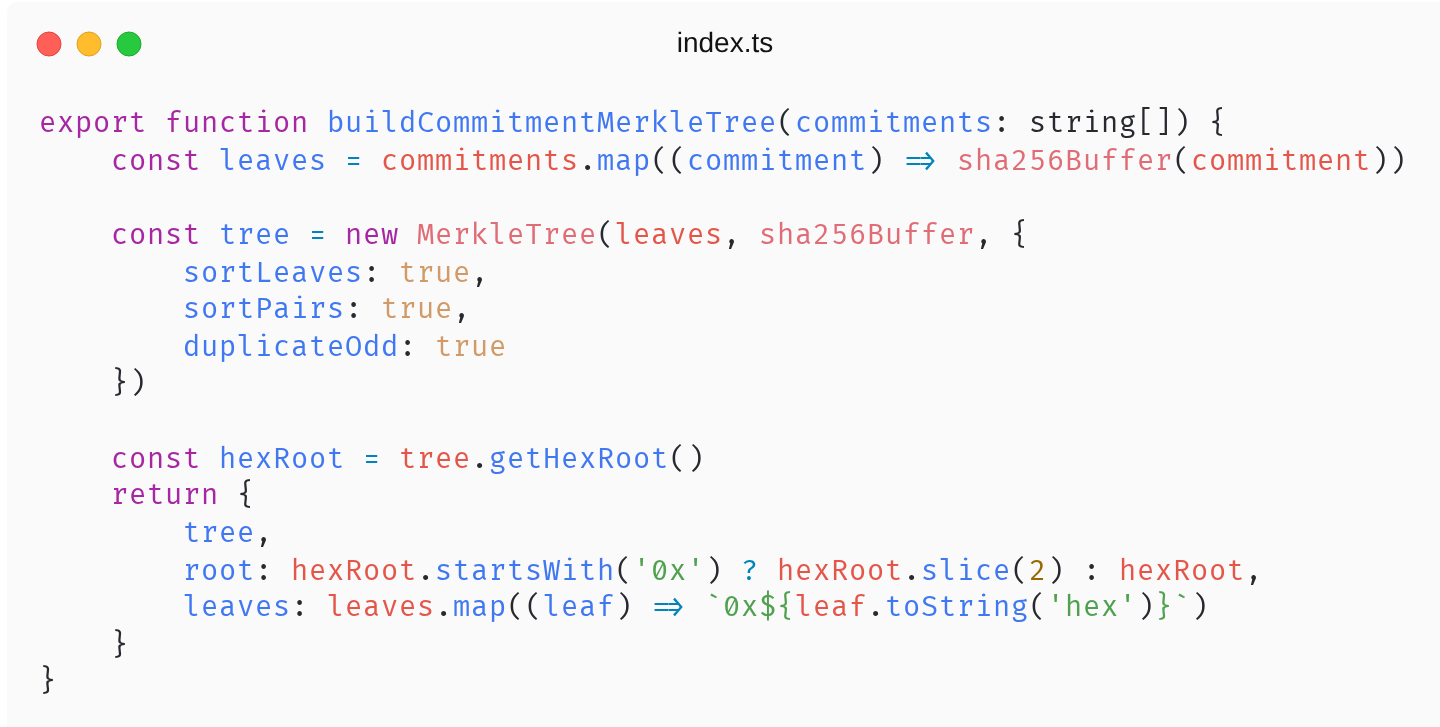
\includegraphics[width=0.85\textwidth, keepaspectratio]{Figures/code/merkle-tree-config.png}
    \caption{Cấu hình \pkg{MerkleTree} của thư viện \pkg{merkletreejs} ở tầng off-chain}
    \label{fig:merkle-tree-config}
\end{figure}

Tùy chọn \texttt{sortPairs: true} phải được phản chiếu nguyên vẹn ở phía chaincode Go. Hàm \pkg{hashSortedPair} trong chaincode (Hình~\ref{fig:hash-sorted-pair-go}) làm chính xác việc đó: so sánh hai dãy byte, gom dãy nhỏ hơn về trước, rồi băm SHA-256 phần nối. Nếu thuật toán này khác giữa hai phía, gốc Merkle on-chain và off-chain sẽ lệch ngay cả với cùng tập phiếu — và toàn bộ luồng kiểm chứng sau đó vô hiệu.

\begin{figure}[H]
    \centering
    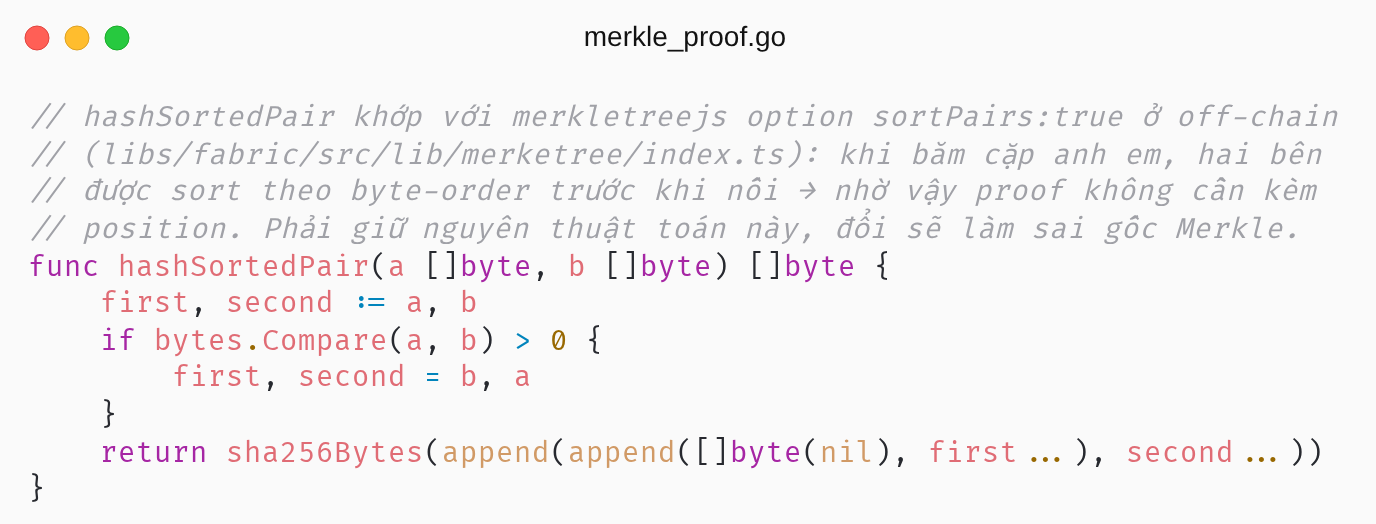
\includegraphics[width=0.85\textwidth, keepaspectratio]{Figures/code/hash-sorted-pair-go.png}
    \caption{Hàm \pkg{hashSortedPair} trong chaincode Go đồng bộ với off-chain}
    \label{fig:hash-sorted-pair-go}
\end{figure}

\subsubsection{Cam kết Merkle root đảm bảo gì}

Sau khi \pkg{commitMerkleRoot} được ghi lên sổ cái Fabric, ba bất biến quan trọng được thiết lập:

\begin{itemize}
    \item \textbf{Snapshot bất biến:} tập hợp phiếu tại thời điểm đóng bầu cử được \textit{đóng băng} trong một giá trị 32 byte. Bất kỳ thay đổi nào trong tập phiếu (thêm, xóa, sửa) đều sinh ra root khác.

    \item \textbf{Bằng chứng thành viên (\textit{membership proof}):} bất kỳ phiếu nào trong cuộc bầu cử cũng có thể tự chứng minh thuộc về tập phiếu chính thức mà không cần tiết lộ các phiếu khác — một dạng \textit{zero-knowledge-like} thực tế nhờ Merkle proof.

    \item \textbf{Đối chiếu chéo DB và chain:} giá trị \pkg{election.merkleRoot} lưu trong MongoDB được đối chiếu với \pkg{MerkleRootView.merkleRoot} đọc từ chain. Bất kỳ chênh lệch nào cũng đồng nghĩa backend đã tự ý thay đổi root sau khi commit — sự việc có thể bị bất kỳ bên kiểm toán nào phát hiện.
\end{itemize}

\subsubsection{Độ phức tạp của bằng chứng Merkle}

Độ dài đường dẫn bằng chứng cho một phiếu trong cây có $N$ lá là $O(\log_2 N)$. Ví dụ: với 1.000 phiếu, đường dẫn dài 10 băm, tổng 320 byte; với 10.000 phiếu, đường dẫn dài 14 băm, tổng 448 byte. Tốc độ kiểm chứng vì vậy gần như không phụ thuộc vào quy mô bầu cử — ngay cả với 100.000 phiếu, bằng chứng cũng chỉ dài 17 băm. Đây là yếu tố cho phép cử tri tự kiểm chứng phiếu của mình trên máy tính cá nhân mà không cần tải về toàn bộ sổ cái.
